\documentclass{article}

% Language setting
% Replace `english' with e.g. `spanish' to change the document language
\usepackage[english]{babel}

% Set page size and margins
% Replace `letterpaper' with `a4paper' for UK/EU standard size
\usepackage[letterpaper,top=2cm,bottom=2cm,left=3cm,right=3cm,marginparwidth=1.75cm]{geometry}

% Useful packages
\usepackage{amsmath}
\usepackage{graphicx}
\usepackage[colorlinks=true, allcolors=blue]{hyperref}

\title{LC circuits}
\author{Gian Laager and Sebastian Rast}

\begin{document}
\maketitle

\section{Introduction}

\subsection{Goal}
\subsection{Hypothesis}

\section{Theoretical Background}
\subsection{How does a LC circuit work?}

\begin{figure}[!ht]
    \centering
    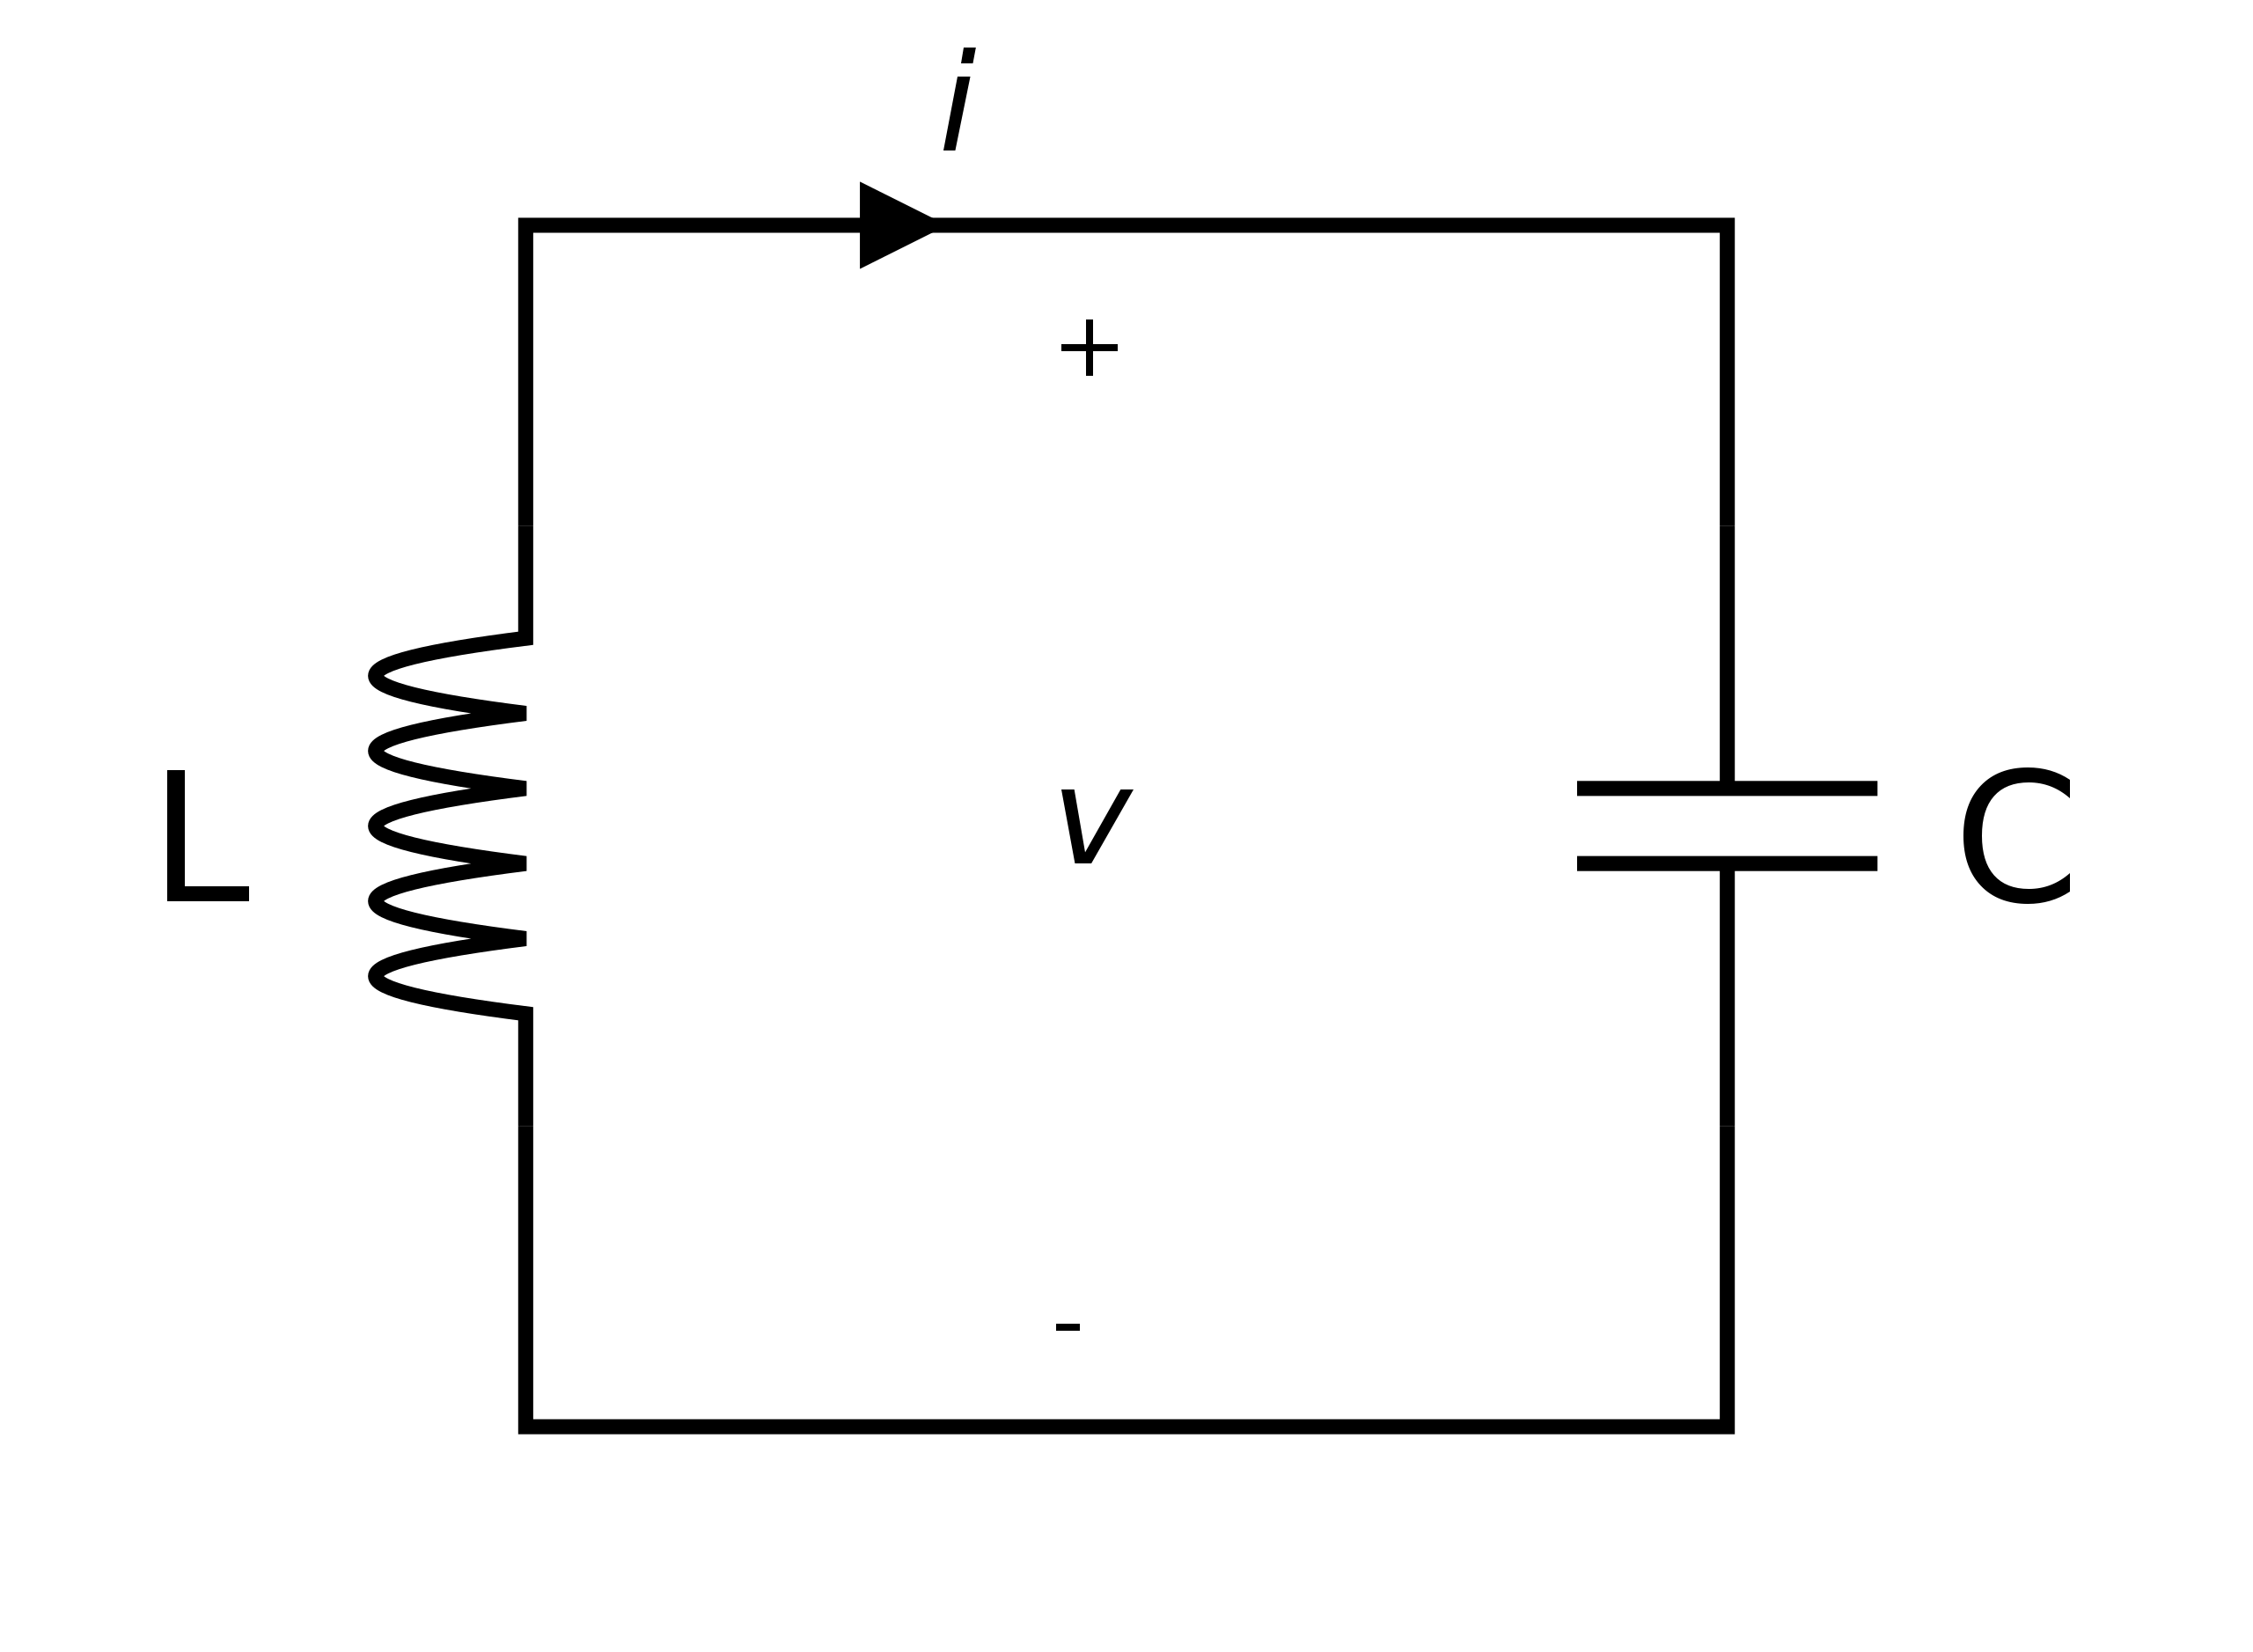
\includegraphics[width=0.6\textwidth]{images/2560px-LC_parallel_simple.svg.png}
    \caption{Schematics of a LC circuit}
    \label{fig:my_label}
\end{figure}

\subsection{Bandstop filter}




\section{Experimental arrangement}
schema

\section{Analysis}

\section{Conclusion}

\bibliographystyle{alpha}
\bibliography{sample}

\end{document}